\def\figtop{\rule{\textwidth}{0.5mm}}
\def\figbot{\rule{\textwidth}{0.5mm}}
\documentclass[11pt, oneside]{article}   	% use "amsart" instead of "article" for AMSLaTeX format

\usepackage{rotating} % for sideways and sidewaystable, etc. environments
% instead, using: see http://www.tex.ac.uk/cgi-bin/texfaq2html?label=landscape
\usepackage{rotfloat}
% the following package, when present, lets the figures and tables orient oppositely on even and odd pages
%
\usepackage{lscape} 
%\usepackage{pdflscape} % see http://en.wikibooks.org/wiki/LaTeX/Page_Layout
%\usepackage{graphpap} % not used after all
\usepackage{caption}
\usepackage{tikz}

\usepackage[margin=1cm]{geometry}                		% See geometry.pdf to learn the layout options. There are lots.
\geometry{a4paper} %{letterpaper}                   		% ... or a4paper or a5paper or ... 
%\geometry{landscape}                		% Activate for rotated page geometry
%\usepackage[parfill]{parskip}    		% Activate to begin paragraphs with an empty line rather than an indent

\usepackage{graphicx}				% Use pdf, png, jpg, or eps§ with pdflatex; use eps in DVI mode
								% TeX will automatically convert eps --> pdf in pdflatex		
\usepackage{amssymb}

%SetFonts

%SetFonts


\title{Brief Article}
\author{The Author}
%\date{}							% Activate to display a given date or no date

\begin{document}
\pagestyle{empty}
%\maketitle
%\section{}
%\subsection{}

\begin{sidewaysfigure}
\centering
%\figtop
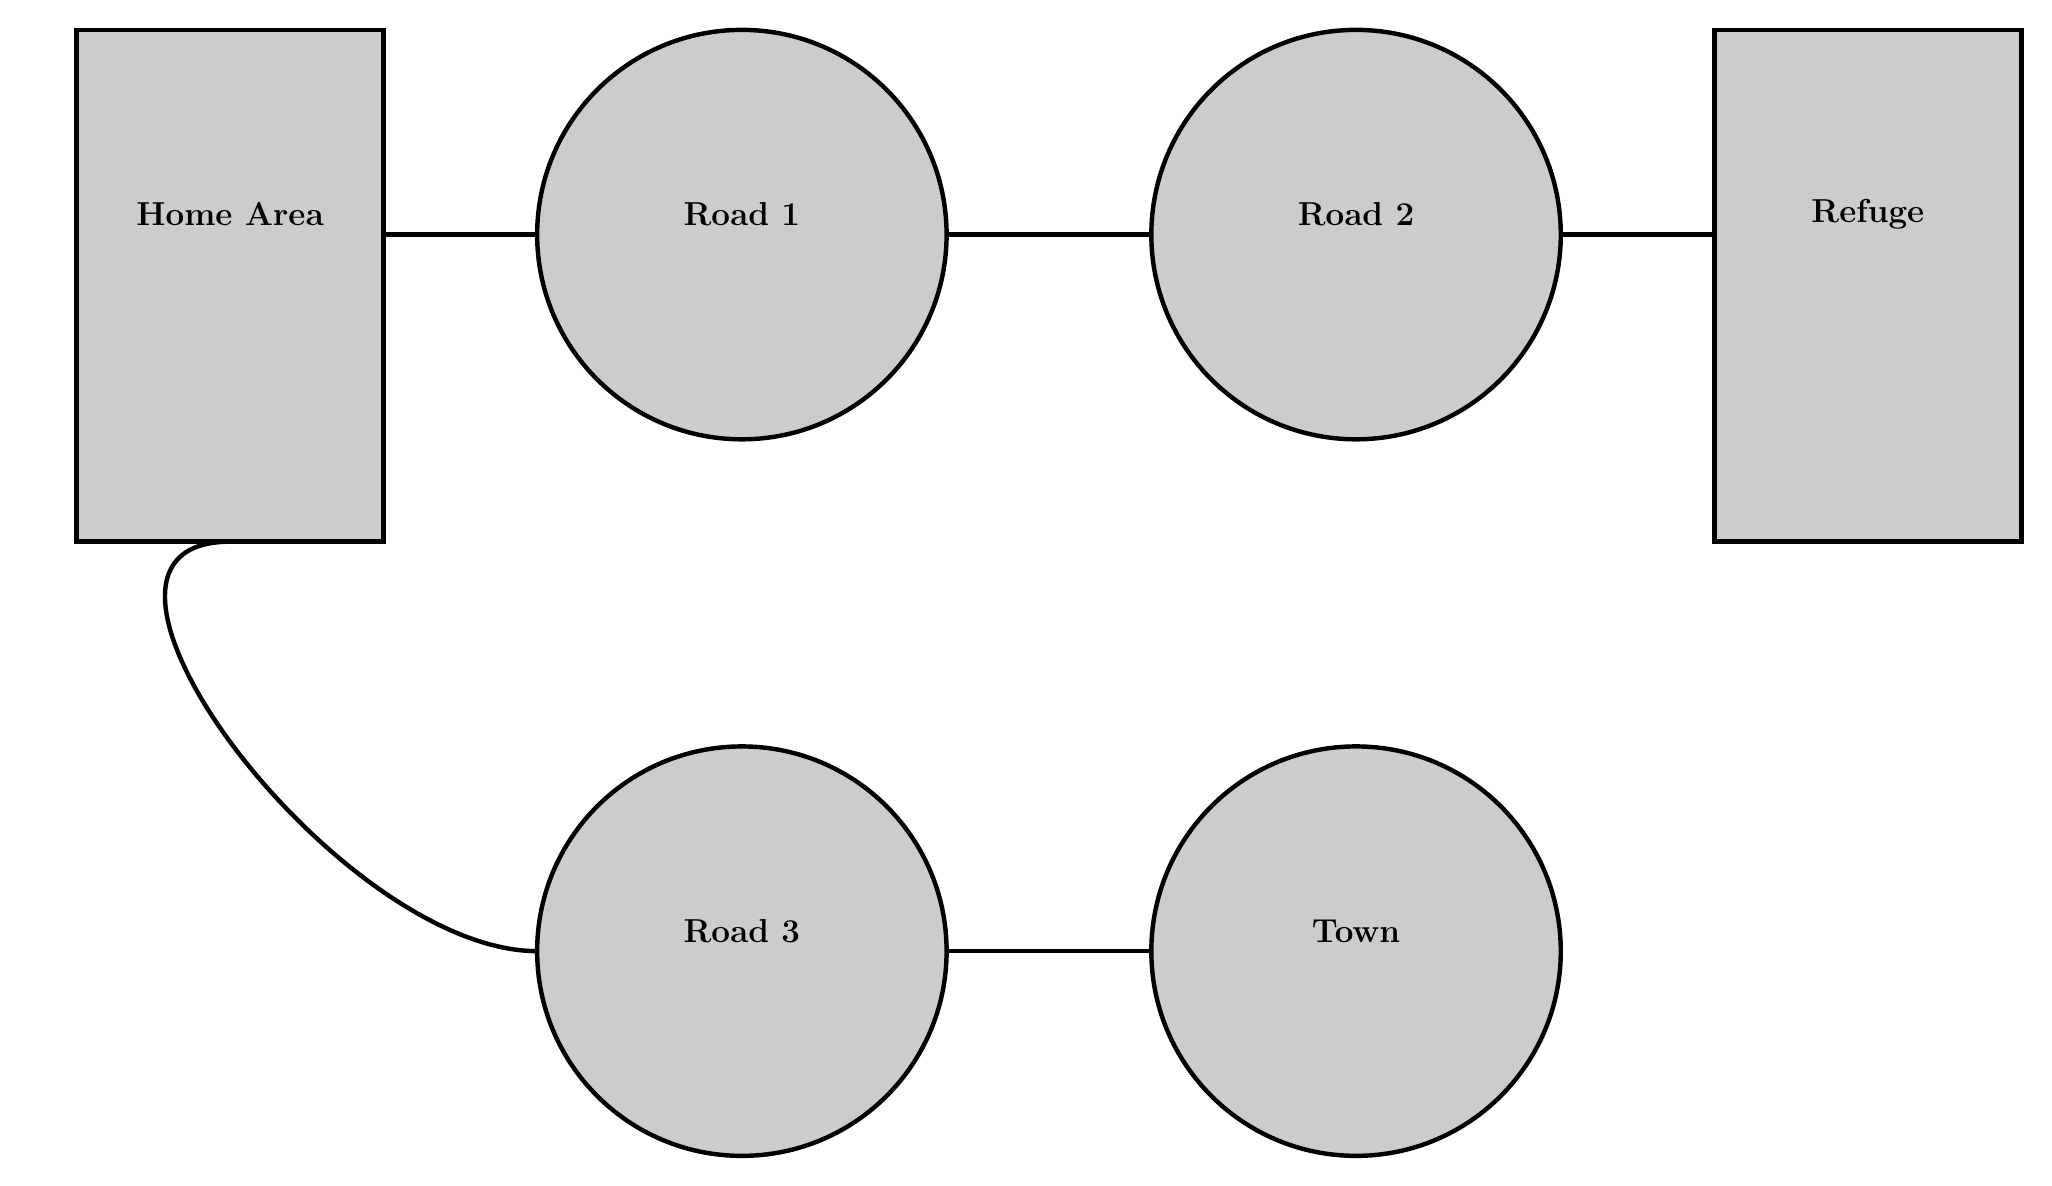
\begin{tikzpicture}[xscale=1.3,yscale=1.3]
%\draw [ultra thick] (3,0.5) circle [radius=0.5];
\draw [fill = gray!40, ultra thick] (0,11) rectangle (3,6);
\node at (1.5,9.2) {\large\textbf{Home Area}};
\draw  [fill = gray!40, ultra thick] (6.5,9) circle [radius=2];
\node at (6.5,9.2) {\large\textbf{Road 1}};
\draw  [fill = gray!40, ultra thick] (12.5,9) circle [radius=2];
\node at (12.5,9.2) {\large\textbf{Road 2}};
\draw [fill = gray!40, ultra thick] (16,11) rectangle (19,6);
\node at (17.5,9.2) {\large\textbf{Refuge}};
% Town and road
\draw  [fill = gray!40, ultra thick] (6.5,2) circle [radius=2];
\node at (6.5,2.2) {\large\textbf{Road 3}};
\draw  [fill = gray!40, ultra thick] (12.5,2) circle [radius=2];
\node at (12.5,2.2) {\large\textbf{Town}};


% The links:
\draw [ultra thick] (3,9) -- (4.5,9);
\draw [ultra thick] (8.5,9) -- (10.5,9);
\draw [ultra thick] (14.5,9) -- (16,9);

% Town links
\draw [ultra thick] (8.5,2) -- (10.5,2);
\draw [ultra thick] (4.5,2) to [out=180, in=180] (1.5,6);

%\draw [help lines] (0,0) grid (19,11); 
\end{tikzpicture}
%\caption{Bob!}
\end{sidewaysfigure}
\end{document}  